
In this section we present the results of a controlled experiment in
which we injected bugs into \moss\ \cite{Schleimer:2003:WLA}, a widely
used plagiarism detection service.  A primary goal of this experiment
was to see whether our algorithm was effective at finding most or all
bugs in an application; thus it was necessary to know the set of bugs
we were looking for.  Both \moss\ source code and bug logs were
available to us, and so we could easily reproduce historical bugs.

We briefly describe the nine bugs we added to \moss.  As discussed in
\Autoref{sec:introduction}, these bugs vary from low-level crashing
bugs to high-level logic bugs that simply produce incorrect output.
Except where noted, these are all bugs that originally occurred in
\moss.
\begin{enumerate}
\item We reintroduced a bug that causes the number of
lines in C-style multi-line comments to be counted incorrectly.  This bug causes incorrect output
in certain circumstances: an option to
match comments must be on (normally \moss\ ignores comments)
and there must be matching multi-line comments that affect the output.

\item We removed a check for a
null {\tt FILE} pointer.  This is not originally a \moss\ bug; it is exactly analogous to the {\tt ccrypt} bug (see \Autoref{sec:revisited}).

\item We removed an array bounds update
in the routine for loading preprocessed data from disk. The
program behaves normally unless the function is called a second time,
in which case previously loaded data may be partially overwritten.
This bug has unpredictable effects and
was particularly difficult to find originally.

\item We removed a size check that prevents users from supplying command-line arguments
that could cause the program to overrun the bounds of an array.

\item For historical reasons, \moss\ handles Lisp programs differently
from all other languages.  We removed a end-of-list check in the Lisp-specific
code.

\item For efficiency \moss\ preallocates a large area of memory for its primary data structure.
When this area of memory is filled, the program should fail
gracefully.  We removed an out-of-memory check. 

\item \moss\ has a routine that scans an array for multiple copies of a data value.
We removed the limit check that prevents the code from searching past the end of the array.  
This bug did not occur in \moss; it is intended to be a more frequently occurring version of bug \#8.

\item  A buffer overrun, this bug was never known to have caused a failure in \moss. It
was discovered originally by a code review.

\item This bug is a variant of bug \#4, but involves a different command-line argument and
a different array.
\end{enumerate}

In summary, six of the nine bugs were originally bugs in \moss, two are variants on \moss bugs, and one
is a port of the {\tt ccrypt} bug.  The bugs
range from typical C coding errors (e.g., \texttt{NULL} pointer dereferences
and array overruns) to high-level violations of a system's internal
invariants (e.g., bugs \#1 and \#3).

To measure the accuracy of our techniques we logged 
when each bug was triggered.  Of course, this logging 
code was excluded from the sampling instrumentation.
To determine whether a run produced correct output we compared it against a run
of the reference version of \moss.  As discussed in \Autoref{sec:introduction},
in practice the labeling of runs as successful or failed is done by either detecting
crashes, internal assertion failures, or (speculatively) by direct user feedback that the output
of the program appears incorrect.  Our use of a reference version in this experiment made
it possible for us to label large numbers of runs automatically.

Table~\ref{tab:exps} shows that \moss\ has over 200,000 instrumented predicates,
and {\tt Rhythmbox} has over 800,000.
The reader may wonder whether it is practical to actually generate a report on
800,000 predicates on a client machine and then upload it to a central
server for analysis.  The answer is definitely yes.  First, recall
that the predicates are synthesized from about half as many counters.
The counters are mostly zeroes and so compress extremely well,
resulting in uploaded files in the range of 10-50Kbytes.

As can be seen in Table~\ref{tab:exps}, the {\tt branches} and {\tt returns} schemes
resulted in short reports.  We again used correlations between predicates to help us navigate
the {\tt scalar-pairs} report.

We briefly summarize the results.
The algorithm identified a highly-ranked cause that would be useful to a programmer
for seven of the nine bugs.  For the two other bugs,
one (bug \#7) occurred in our experiment but never caused
the program to crash or produce incorrect output; the other (bug \#8) was never
triggered at all.  There is no way our algorithm can find causes of bugs that do not
occur, but recall that part of our purpose in sampling user executions
is to get an accurate picture of the most important bugs. It is consistent with
this goal that if a bug never causes a problem, it is not only not worth fixing,
it is not even worth reporting.

% CHECK
In more detail, we examined the reports generated with \nicefrac{1}{100} downsampled data.
The branches report has 4 predicates with a 1.0 fail rating:
%%
\begin{verbatim}
Predicate      Context    Increase   Failure
strcmp(s,"lisp") == 0  
               0.11       0.89       1.00
*pstart + numpassages > pmax - 1 
               0.10       0.85       0.95
strmp(argv[i],"-p") == 0
               0.11       0.83       0.93
strmp(argv[i],"-s") == 0
               0.11       0.43       0.53
config.dbfile != NULL
               0.03       0.47       0.50
\end{verbatim}


\begin{verbatim}
0.94 Inc, 1.00 Cr, 0.06 Co, process_file_pass2 line 5523
0.80 Inc, 1.00 Cr, 0.20 Co, handle_options line 5742
0.80 Inc, 1.00 Cr, 0.20 Co, string2lang line 4366

0.78 Inc, 1.00 Cr, 0.22 Co, handle_options line 5789
\end{verbatim}

Each line of a report lists the increase, fail, and context scores of
a predicate, as well as the function name and line number where it
occurs.  We have dropped some fields of the report (such as the text
of the predicate itself and the number of failing and successful runs
in which the predicate is observed) to avoid clutter.

The first predicate listed does not immediately suggest what the cause
of failure might be. By looking at the failure log, we see that this predicate
is highly correlated with a subset of the runs in which bug \#1 is
triggered; an engineer with a deep understanding of how \moss\ works
might be able to figure out the bug from this predicate alone.
The next three predicates are obvious ``hits.''  The second predicate
tests whether comment matching should be turned on, and if it is turned on the program is
guaranteed to fail. This is a much more obvious cause for bug \#1, and the predicate points directly
to the fact that something is wrong in the comment matching
code.\footnote{Recall that bug \#1 is non-deterministic; why then is
  the crash score 1.0?
The discrepancy is the result of sampling error.  In the full data set
(with \nicefrac{1}{1} sampling) the crash measure for this predicate is indeed
only 0.88.}
The
next predicate marks the test in the code that decides whether \moss\ is analyzing Lisp
programs; the crash score of 1.0 tells us that whenever a Lisp program is
processed, \moss\ crashes.  The fourth predicate
is an obvious cause of
bug \#6; it reveals that whenever the amount of memory to use is set
via a command line option, the program will crash.  (The full data set shows that bug \#6 is non-deterministic with respect to this predicate, so once again the certainty that the program will crash is the result of sampling error.)  All three of these predicates illustrate the potential of our method to
help pinpoint the root cause of a crash rather than just where the crash
happened.  Each of these predicates immediately suggests
what test case to try to reproduce the bug.

The 9th listed cause in the branches report says that whenever the
user supplies the command line option to write a database, the chance
of failure jumps to 62\% (bug \#2), and the 14th ranked cause says
that whenever a database is read the chance of failure is 55\% (bug
\#3).  All the other causes between the 5th and 21st in the branches
report are predicates that also implicate one of bugs 1, 2, 3, 5, or
6.  Below the 22nd listed cause the $\increase(\ldots)$ scores drop to
1\%; we did not examine these predicates.

The returns report is also quite interesting.  Recall that this
instrumentation scheme samples the return values of functions (whether
they are negative, positive, or zero).  The first two entries in this
report are the results of string comparisons that point directly to bug
\#5.  The third entry is the {\tt open} call in the function that writes
a database; the predicate shows that when this function returns {\tt NULL},
the program is guaranteed to crash (i.e., 1.0 crash score).  This is the
cause of bug \#2.

The fourth entry of the full data (not the \nicefrac{1}{100} downsampled data)
returns report is very interesting.  This predicate shows that one of
the file read operations in the function that loads a database can
fail, and when it does \moss\ itself fails with probability 0.64.
It turns out that \moss\ assumes that any database it reads has the
correct database file format, because it does no checking to ensure
that the read operations that actually load the database succeed.  This is a previously
unknown bug in \moss.  It is a bit surprising that this bug was detected,
because a run is only labeled a failure in our experiment if the
reference \moss\ and the buggy \moss\ differ in their outcome, and
this bug is present in both versions.  Thus, this bug could only be detected
when another one of the introduced bugs was also triggered in the same
run and caused the buggy version of \moss\ to fail in a different way.
This explains the very low $\increase(\ldots)$ score for this
predicate (the chance of failure only increases by 11\% when this bug
occurs) and why it was not observed in the \nicefrac{1}{100}
downsampled data.  With enough runs it would be observed at
any sampling rate, but the anomaly that the reference and buggy
versions of \moss\ share this bug means that, at the
\nicefrac{1}{100} sampling rate, many more runs are likely needed
than what we had for this experiment.

Bugs \#4 and \#9 have no causes in either the branches or the returns
reports, as they are not correlated with any branch nor with the
result of any function call.  In the \nicefrac{1}{100} downsampled
scalar-pairs report, there are obvious causes showing that the array
bounds have been exceeded which are ranked 26th (for bug \#4) and 52nd (for bug
\#9).  In both cases it didn't matter which predicate we chose to
represent the bug for the line identified as the cause of the bug; all
of the predicates were essentially the same.  The other
predicates ranked higher than 52nd in the scalar-pairs report are
either more obscure, but more deterministic, indicators for bug \#4 or
for one of the other five observed bugs.  Given the emphasis on
determinism in our ranking function, bug \#9 could not be listed
higher, as it is the most non-deterministic bug in our data set with a
$\crash(\ldots)$ score of 0.72.

Finally, we compared the reports generated from \nicefrac{1}{100} sampled data
with the reports generated from \nicefrac{1}{1} sampled data.  The reports were
similar, but not identical.  In particular, the ordering of the
predicates was slightly different and a few predicates with relatively
few observations or a low $\increase(\ldots)$ score --- and thus high
sensitivity to whether one or two successful or failing runs were
observed or not --- appeared on
%one list and not the other.
the \nicefrac{1}{1} list but not the \nicefrac{1}{100} sampled list.

In summary, our algorithm did a good job of producing concise reports that not
only identified the bugs, but also gave useful information about the root causes and
how to reproduce the bugs.  In addition, the algorithm identified a previously unknown
bug.

\subsection{Effect of Sampling on Predicate Selection}

We now examine the effect of the sampling rate and the number of
program trials on the number of predicates that are retained by step
(1) of the algorithm.
We start with $3000$ randomly
selected trial runs, and add $3000$ random trials at a time, until we
incorporate all $31,875$ runs of our data.  We record the number of
predicates retained at each step.  This process is repeated ten times
for each sampling rate, with ten different random permutation sequences
of our data. We plot the mean and the confidence interval (one
standard deviation above and below the mean) in
\Autoref{fig:predkept-a}.  Using all $31,875$ trial runs, we retain $1178$ 
predicates when the data is not sampled (i.e.,\ sampling rate is 
$\nicefrac{1}{1}$), $917$ at sampling
rate $\nicefrac{1}{10}$, $851$ at $\nicefrac{1}{100}$, and $548$ at
$\nicefrac{1}{1000}$.

\begin{figure}
\centering
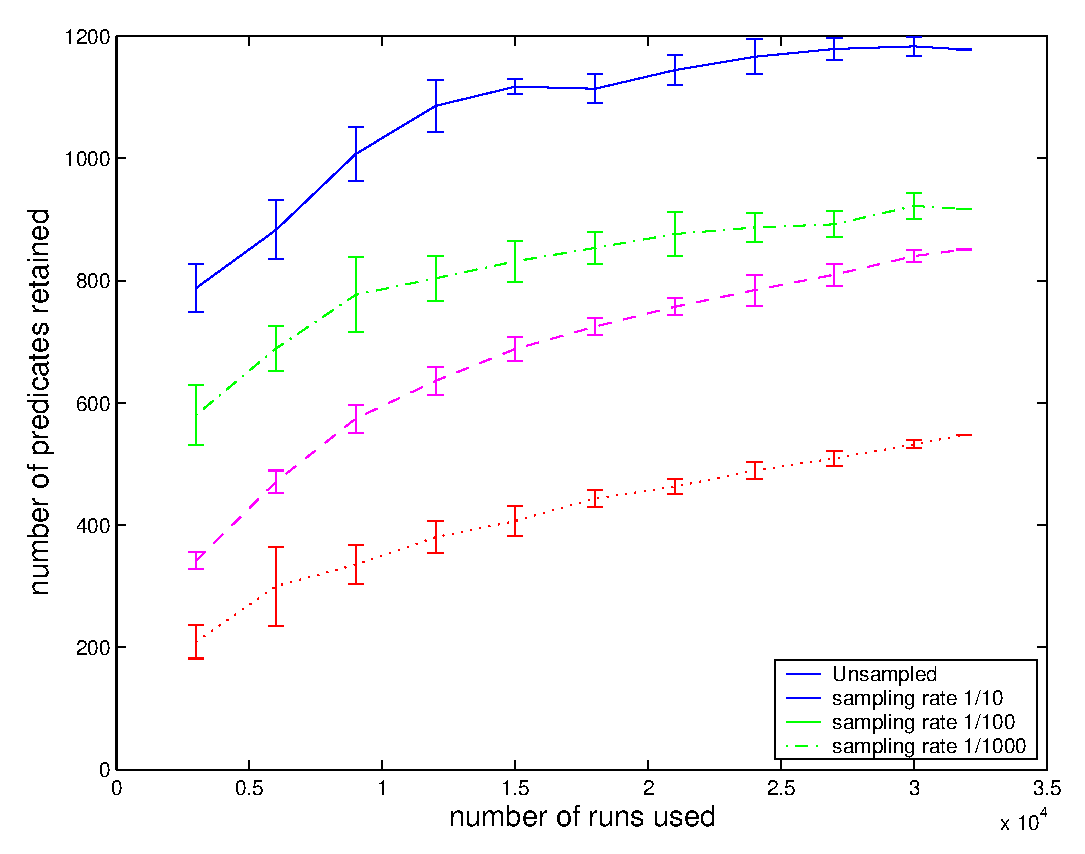
\includegraphics[width=\columnwidth]{predkept3a}
(a) Branches, returns, and scalar-pairs. \\
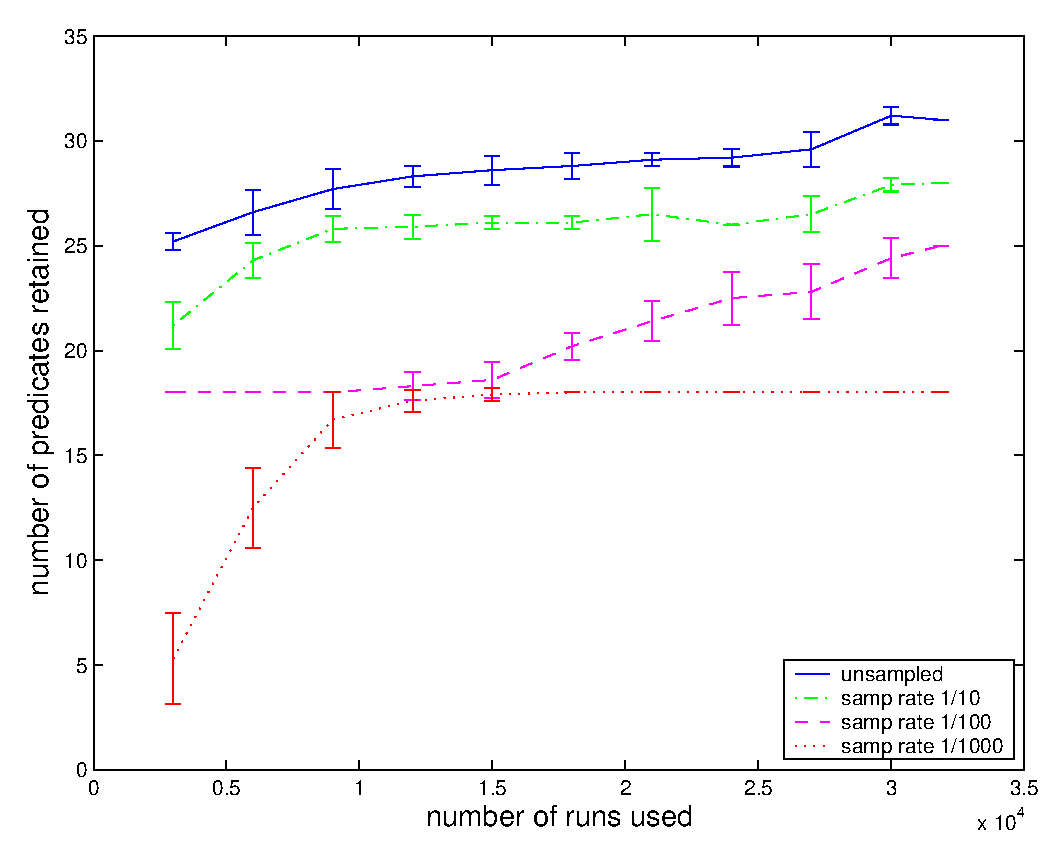
\includegraphics[width=\columnwidth]{predkept3b}
(b) Branches and returns only.
\caption{The effect of sampling and data size on the number of
  predicates selected.}
\label{fig:predkept}
\end{figure}

Two trends are apparent from \Autoref{fig:predkept}.  As one would expect,
the number of retained predicates decreases as the sampling rate decreases,
and increases as more trial runs are included.  If we had an unlimited number
of trial runs, the number of retained predicates at all sampling rates should
approach the result with no sampling.  

Note also that increasing 
the number of trial runs always seems to increase the number of retained 
scalar-pairs predicates, whereas the branch and returns predicates run into 
a plateau at lower sampling rates.  Though there may not be much significance 
in this discovery, we conjecture that it is due to the fact that scalar
pairs predicates are much more often observed than the other two kinds of
predicates.  Therefore determining the importance of scalar pairs predicates
takes much fewer sampled trial runs.

%% As is apparent from the graph, there is much larger variation in the
%% number of selected predicates when we use fewer trial runs.
%% %Using $3000$ trials, at the minimum we
%% %retain $7429$ predicates using unsampled data, $7654$ when sampling
%% %rate is $\nicefrac{1}{10}$, $7347$ at $\nicefrac{1}{100}$, and $6750$
%% %at $\nicefrac{1}{1000}$;
%% As we incorporate more examples of successful and failed \moss\ runs,
%% the variances decrease for all sampling rates, but the means behave
%% somewhat differently.  When the data is not sampled, the average
%% number of selected predicates stays around $8100$ for all data sizes.
%% Sampling adds noise to this procedure.  As we observed previously,
%% a moderate sampling rate tends to drive up the $\increase(\ldots)$ scores, and
%% thus enlarges our set of selected predicates (except when we are using
%% very few trial runs).

%% At the relatively high sampling rate of
%% \nicefrac{1}{10}, there are still enough samples taken at most
%% instrumentation sites, and there is a net increase in the number of
%% selected predicates.  Once the sampling rate shrinks to
%% \nicefrac{1}{100} and below, however, the effect of sparse
%% sampling sets in.  Fewer samples are taken overall on fewer predicates,
%% and as a result, fewer predicates have a nonzero $\increase(\ldots)$ score.
%% Incorporating more runs tends to alleviate the situation; at above
%% 10,000 runs, roughly the same number of predicates are retained for
%% the \nicefrac{1}{100} sampled data as the complete data.  The very
%% sparse sampling rate of \nicefrac{1}{1000}, on the other hand,
%% causes much more change in the final result.  A lot more predicates
%% are eliminated when using fewer trials, and a lot more predicates are
%% retained using more trials.

%% Most of the volatility in the results come from the scalar-pair
%% predicates.  \Autoref{fig:predkept-b} shows the same graph for
%% only the branch and return predicates.  Here, across all data sizes,
%% the number of selected predicates remains roughly constant at each
%% sampling rate.  The complete data is still able to select the fewest
%% number of predicates, with \nicefrac{1}{100} sampled data following
%% close behind.  The \nicefrac{1}{1000} sampled data still produces a
%% net increase in the number of selected predicates.

%% LocalWords:  downsampling lang downsampled predelim predkept
